\documentclass[a4paper]{jsarticle}

\usepackage{txfonts}
\usepackage[expert, deluxe]{otf}
\usepackage{redeffont}
\usepackage[dvipdfm]{graphicx}

\title{ソフトウェア構想・設計について}
\author{情報環境プロジェクト3班 \\
ソフトウェア担当}
\date{\today}

\begin{document}
\maketitle

3班がソフトウェア開発を行った際に,どのようにしてシステムを設計したかを順を追って説明する.

\section{要件定義}
テーマ設定をもとにチーム内で議論した結果,制作するシステムには最低限以下の機能が必要であるという結論が得られた.
\begin{itemize}
\item 個人情報の登録機能
  \begin{itemize}
  \item あらかじめ個人の障害の程度などの情報を登録しておき,容易に検索・施設情報の照会を行うことができるようにする
  \end{itemize}
\item 施設情報の検索機能
  \begin{itemize}
  \item キーワードから施設を検索
  \item 自分の障害の程度と施設情報から導き出した施設の利用可能性による検索結果のソーティング
  \end{itemize}
\item 個人情報を考慮した施設のバリアフリー情報表示
  \begin{itemize}
  \item 検索を行った人にとって,施設が利用可能かどうかを表示する
  \item 施設が利用できない場合,何が原因で利用できないかを表示する
  \end{itemize}
\item 施設への情報のフィードバック機能
  \begin{itemize}
  \item 利用者が感じたことを施設に知らせるための機能
  \item 施設情報のページに意見を書き込める掲示板を設置する
  \end{itemize}
\end{itemize}

\section{必要なコンポーネントの洗い出し}
次に,前節で定義した要件を実現するために必要なコンポーネントを洗い出した.
今回のシステムに登場するコンポーネントは,大きく分けるとサーバとクライアントの2つになる.

クライアントサイドではウェブブラウザが動作しており,サーバから受信したHTMLファイルや画像ファイルをもとに,ユーザインターフェースを構成する.
また,ブラウザ上で動作するプログラミング言語の JavaScript を用いる事によって,動的なサーバと通信や動的なインターフェースの書き換えを実現することができる.

サーバではファイルシステム・DBサーバ・セッションストア・ウェブサーバが存在しており,それぞれ役割が異なっている.
ファイルシステムは基本的に変更されることのない情報を保有している.HTML ファイルや, JavaScript などプログラムのソースファイルはこのファイルシステム上に保管されている.
DBサーバは,店舗情報やユーザ情報など,多くのデータの中から目的のデータを検索して見つけることが必要とされるようなデータを保有している.
セッションストアには,ユーザがログインしているか否かの情報など,一時的に保存され期限が過ぎると削除されるデータが保存されている.
ウェブサーバは,クライアントと通信を行う.上記に述べたデータを取得したり,データベースから検索したりするプログラムがウェブサーバ上で動作し,それらの指示によりクライアントサイドに送信するデータを構築し,実際に送信する.

以上のような役割を果たすコンポーネントが必要である.
今回は工期を短縮するために,各種コンポーネントを選択する上で,いくつか構成上の工夫を行った.
ここでは,その工夫と得られた結果を記述する.
\begin{itemize}
\item クライアントサイドで表示されるユーザーインターフェースを静的なHTMLで作り込むのは大変手間がかかるので,Ajaxの技術を用い,コンテンツを動的に生成するような仕組みにした
  \begin{itemize}
  \item 既存の豊富なライブラリ資源 (jQueryおよびそのplugin, Google Maps API) を活用した.結果として,自作のコード部分を1100行程度に抑えることができた
  \item クライアントサイドでユーザーインターフェースを構築することにより,ページ遷移を伴わない,直感的でわかりやすいインターフェースを実現することができた
  \end{itemize}
\item 将来的に膨大なデータを取り扱うことが考えられるので,データベースソフトとして MySQL を用いた
\item クライアントサイドからのリクエストを解釈し,データベースからデータを取り出し加工するプログラムはPHPで書くことにした
  \begin{itemize}
  \item PHP はウェブアプリケーションの制作に特化した言語で,便利なライブラリが多数用意されており,容易に開発を行うことができた
  \item PHP から MySQL へのアクセスも非常に容易に行うことができる
  \end{itemize}
\end{itemize}

\begin{figure}[htbp]
  \centering
  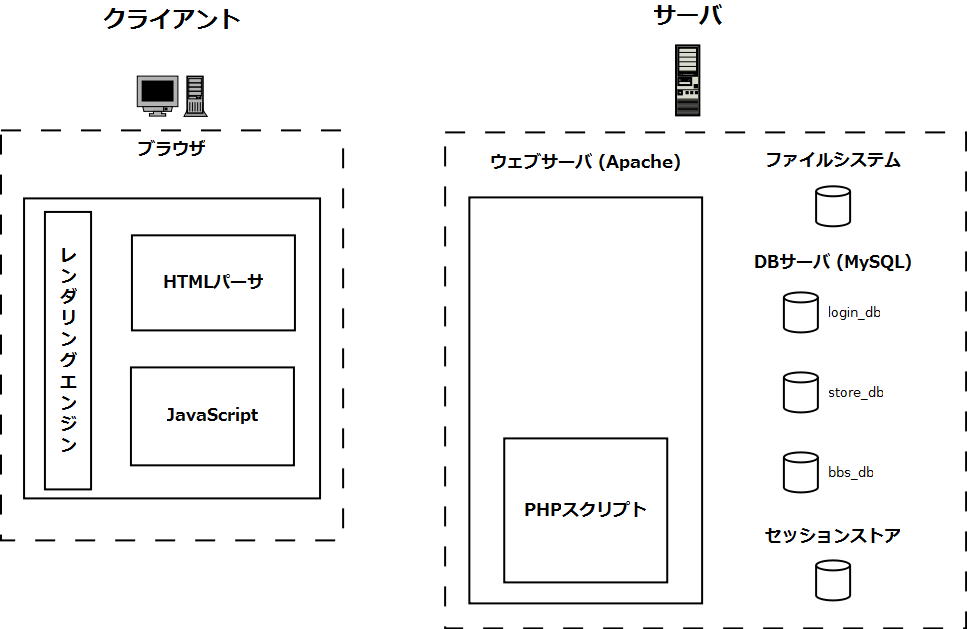
\includegraphics[width=0.8\linewidth]{../../image/story/base}
  \caption{用いたコンポーネント一覧}
  \label{fig:component}
\end{figure}


\section{コンポーネント間の相互作用}

必要なコンポーネントが洗い出せたので,実際にそれらがどのように相互に働きあってシステムを実現するかを考えた.
今回登場するコンポーネントを図~\ref{fig:component}に示す.これらのコンポーネントがどのように相互作用して,ページの表示,ログイン,施設検索,施設詳細情報の表示を実現しているかを解説する.

\subsection{ページの表示}
利用者がこのシステムにアクセスすると,検索語を入力するページが表示される.
このページは,単純なHTMLファイルといくつかの画像,システムのほとんどの動作を担うJavaScriptで書かれたプログラムの3つから構成されている.

\begin{figure}[htbp]
  \centering
  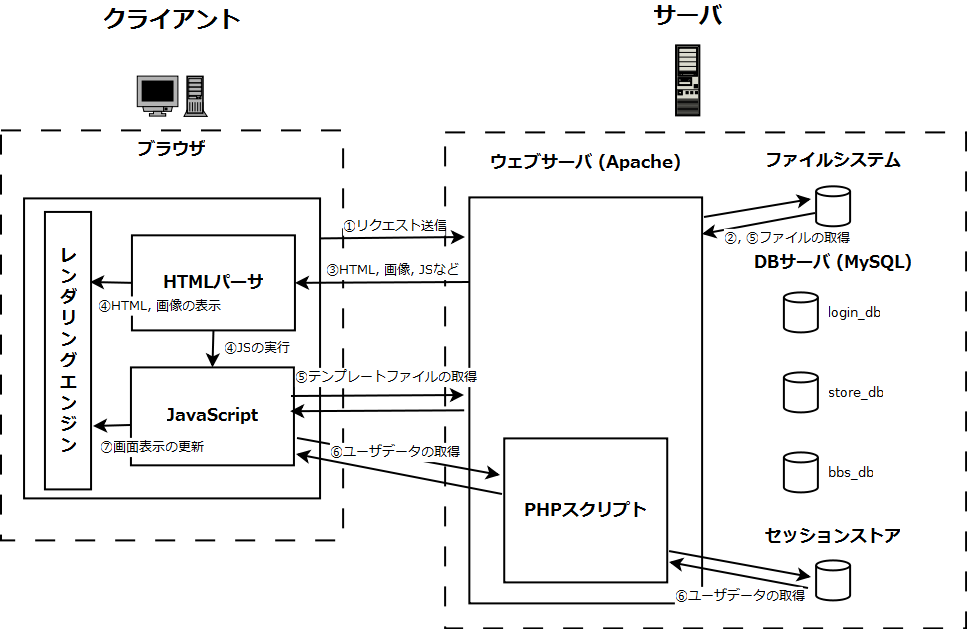
\includegraphics[width=0.8\linewidth]{../../image/story/1_show_page}
  \caption{ページが表示されるまで}
  \label{fig:show_page}
\end{figure}

このページが表示される際にどのような処理が行われるかを,図~\ref{fig:show_page}を用いて説明する.
\ajMaru{1}まず,利用者がブラウザでサイトにアクセスする (サーバにリクエストを送る) と,\ajMaru{2}HTTPサーバ (Apache) はサーバのファイルシステムからリクエストされたファイルの内容を取得し,\ajMaru{3}クライアントにそれらを送信する.
\ajMaru{4}クライアントサイドであるブラウザは,受信したHTMLファイルや画像ファイルをもとに画面表示を更新し,それと同時に受信した JavaScript プログラムを実行する.
\ajMaru{5} JavaScript プログラムは受信したデータを HTML に変換するために用いるテンプレートファイルをサーバから取得し,\ajMaru{6}それと同時にログイン状況の表示や検索条件の初期値を設定するために用いる個人登録された情報をサーバにリクエストする.
このとき,サーバには Cookie に書き込まれたセッションIDが送られる.
サーバは受け取ったセッション ID に対応するユーザ情報がセッションストアに存在するのであれば,ユーザ情報を取得することができそれをレスポンスとして返す.
セッションストアに存在していないのであれば,その旨をレスポンスとして返す.
\ajMaru{7}サーバからユーザ情報が返ってきた場合,ユーザはログインしていると判断できる.ユーザ情報をテンプレートに入力し,「ようこそ○○さん」というメッセージを表示する.ユーザ情報が返ってこなかった場合,ユーザはログインしていないと判断できるため,ログインを促すメッセージを表示する.

\subsection{ログイン}
\begin{figure}[htbp]
  \centering
  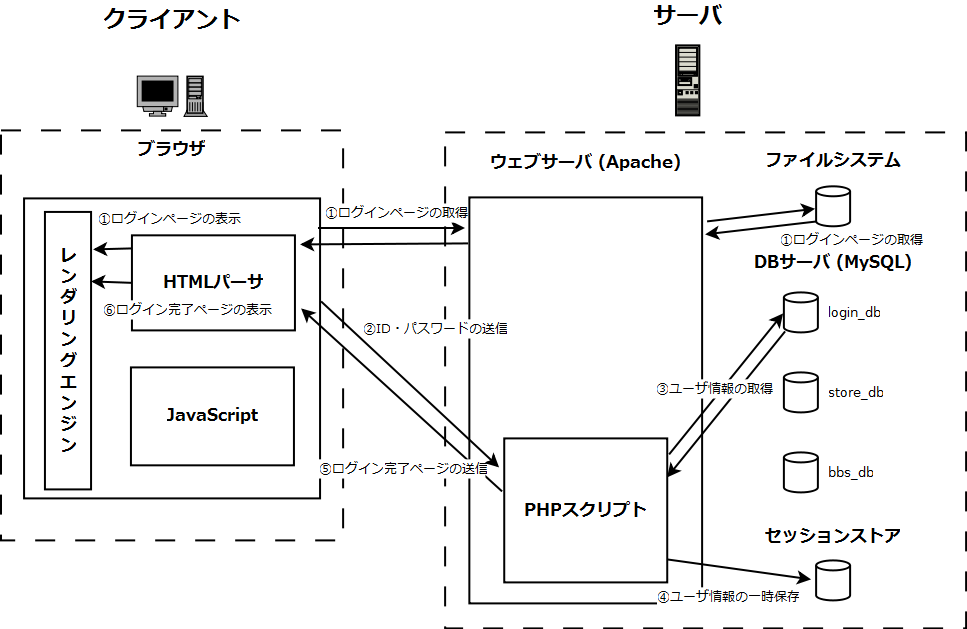
\includegraphics[width=0.8\linewidth]{../../image/story/2_login}
  \caption{ログイン}
  \label{fig:login}
\end{figure}

ログインは古典的なウェブサイトでよくつかわれているような,ページ遷移を伴う処理として実装する.実際の動作を図~\ref{fig:login}を用いて説明する.
\ajMaru{1}ログインページにアクセスすると,サーバからHTMLファイルが送られてきて,ログイン画面が表示される.
\ajMaru{2}ログイン画面にID, パスワードを入力し送信すると\ajMaru{3}サーバ上のPHPスクリプトがデータベース login\_db にクエリを送信し,該当するユーザが存在するか調べ,存在するのであればユーザ情報を取得できる.
\ajMaru{4}ここで取得したユーザ情報を後の利用のためにセッションストアに一時保存し,\ajMaru{5}ログイン完了ページをクライアントに送信し,\ajMaru{6}画面にログイン完了と表示される.

\subsection{施設検索}
\begin{figure}[htbp]
  \centering
  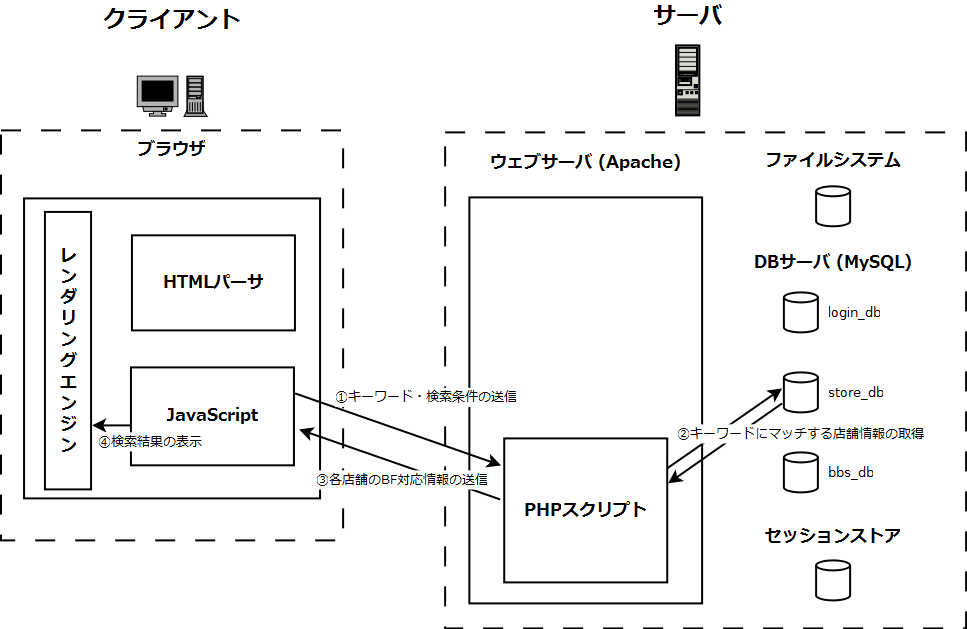
\includegraphics[width=0.8\linewidth]{../../image/story/3_search}
  \caption{施設検索}
  \label{fig:search}
\end{figure}
\ajMaru{1}ユーザが検索キーワードと検索条件を入力し,「検索」ボタンを押すと,クライアントサイドで実行されているJavaScriptがサーバに検索に必要な情報を送信する.
\ajMaru{2}受け取った情報をもとに,サーバ上のPHPスクリプトがデータベースより条件に合致する施設の一覧を取得し,各店舗のより利用が容易であると考えられる店舗から順番に並べ,\ajMaru{3}クライアントサイドに送信し,\ajMaru{4}クライアントは受け取った結果を整形し,出力する.

\subsection{施設詳細の表示}
\begin{figure}[htbp]
  \centering
  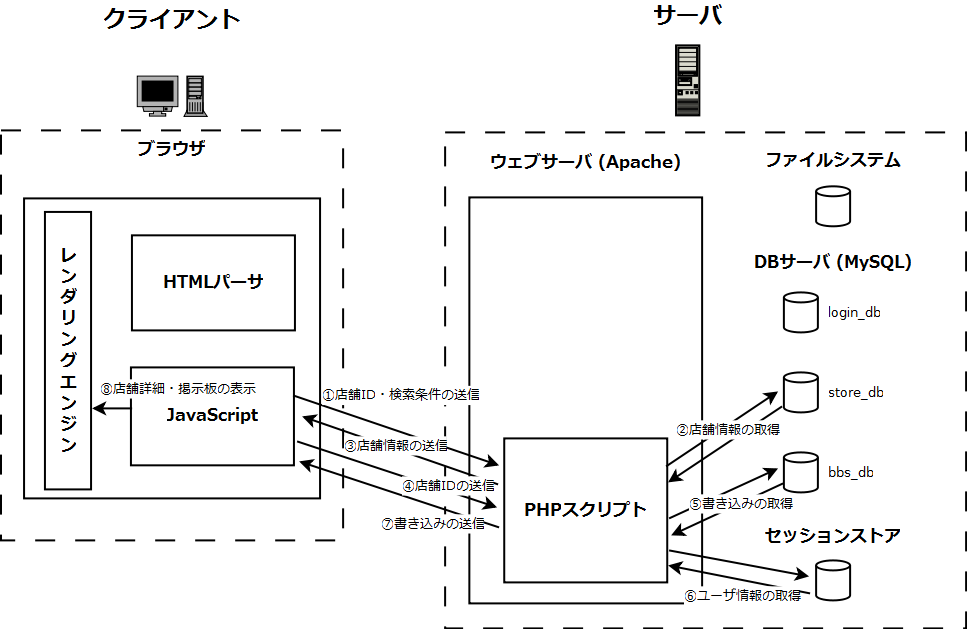
\includegraphics[width=0.8\linewidth]{../../image/story/4_detail}
  \caption{施設詳細の表示}
  \label{fig:search}
\end{figure}
施設検索とほぼ同じである.
施設詳細情報と掲示板への書き込み情報をそれぞれ別個に取得しているので施設検索と比較して矢印の本数が増えている.

\section{各自の作業分担}
各自が他の人の進捗状況に左右されず,待ち時間なく同時並行的に作業を行えるようにするため,システムをある程度まとまった大きさの独立したモジュールに分割し,各自がそれぞれの部分を担当するようにした.
各自の担当は以下のように定めた.

\begin{description}
\item[中島] $\cdots$ クライアントサイド全般, 掲示板関連 (掲示板用PHPスクリプト, \texttt{bbs\_db})
\item[大野] $\cdots$ ログイン関連 (ログイン用PHPスクリプト, \texttt{login\_db})
\item[須田] $\cdots$ 検索関連 (検索用PHPスクリプト, \texttt{store\_db})
\end{description}

\section{通信仕様の策定}
各個人の作業の独立性を担保するために,唯一他の作業分野の影響を受ける部分である
モジュール間でのデータのやりとりの仕方 (データフォーマット・送信する内容) について定めた.
今回はJavaScriptとPHPからの取り扱いのしやすさを考慮して,JSONというフォーマットを採用することにした.
JSONフォーマットは,データ型として文字列・真偽値・数値・配列・連想配列をサポートしており,実際にやりとりされるデータの内容はこれらの型で表されるものに限定した.

\section{システムの実装}
以上の仕様策定をもとに,システムの実装を行った.
作業量,進度の関係で各個人の作業範囲を若干変更したところはあったが,誰かの作業が終わらないせいで自分の作業ができない,という事態にはならず,各作業を独立したモジュールに分割したことの効果が現れていたと考えられる.

\end{document}

%%% Local Variables: 
%%% mode: japanese-latex
%%% TeX-master: t
%%% End: 
